\documentclass[11pt]{article}

\usepackage[a4paper,margin=1in]{geometry}
\usepackage{setspace}
\usepackage{amsmath}
\usepackage{booktabs}
\usepackage{tabularx}
\usepackage{graphicx}
\usepackage{caption}
\usepackage{subcaption}
\usepackage{pdflscape}
\usepackage{placeins}
\usepackage{xurl}
\usepackage[hidelinks]{hyperref}
\usepackage[backend=biber,style=authoryear,maxcitenames=2,maxbibnames=99,natbib=true,giveninits=true,uniquename=false]{biblatex}

\addbibresource{references.bib}
\setcounter{biburllcpenalty}{9000}
\setcounter{biburlucpenalty}{9000}
\setcounter{biburlnumpenalty}{9000}
\graphicspath{{figures/}}
\onehalfspacing
\setlength{\parindent}{1.2em}
\setlength{\parskip}{0pt}

\title{\textbf{Local Scaling and Temporal Learning in Chart-Based Return Prediction}}
\author{Authors omitted for double-anonymized review}
\date{July 2026}

\begin{document}
\maketitle

\begin{abstract}
We study whether chart-based return prediction reflects the chart image itself or flexible learning from recent market histories. In U.S. equities, we compare a chart-based convolutional neural network, a one-dimensional convolutional network trained on locally scaled temporal sequences, and a multimodal model that combines both encodings. The design keeps the universe, windows, horizons, ranking rule, portfolio construction, weighting schemes, transaction costs, and sample splits fixed while varying the representation of the same underlying price and volume history. Image-style high-low scaling is economically central. A sequence CNN using the same local scaling recovers most of the chart-CNN performance, contributes the most stable incremental content in encompassing regressions, and performs especially well when longer input windows are used for short-horizon forecasts. Multimodal fusion performs strongly but delivers limited gains over the best single branch, consistent with substantial overlap between chart and sequence information. Learned models outperform transparent price-based benchmarks most clearly in equal-weighted weekly portfolios. That edge narrows under transaction costs, value-weighting, tradability filters, and the 2020--2024 extension period. The evidence points to a powerful short-horizon signal carried by locally normalized recent market histories, with implementation value concentrated in the less liquid tail of the cross-section.
\end{abstract}

\noindent\textbf{Keywords:} return predictability; chart CNN; local scaling; temporal convolution; technical analysis; transaction costs

\noindent\textbf{JEL classification:} C45; C53; G11; G12; G14

\section{Introduction}

Chart-based return prediction raises a basic interpretation question. When a machine learns from a market chart, what has it learned? A strong chart-CNN portfolio can reflect visual layout, local scaling, flexible learning from recent price and volume data, or a mixture of these channels. The answer shapes how we read evidence from image-based models in empirical asset pricing.

The chart image is the end product of several design choices. A recent market-history window is selected, prices and volumes are normalized within that window, and the normalized path is rendered into a two-dimensional object. A convolutional neural network then learns from the resulting image. Strong performance therefore does not identify the channel behind the signal. The image may contain distinct visual structure. The local high-low scaling may make the signal easier to learn. A flexible model may recover a broader short-horizon price-history pattern that can also be represented as a numerical sequence.

We separate these channels in U.S. equities by comparing three learned model families. The first is a chart-based convolutional neural network trained on price and volume images. The second is a one-dimensional convolutional neural network trained on temporal sequence inputs constructed from the same open, high, low, close, moving-average, and volume histories. The main sequence specification uses the same local high-low scaling embedded in chart construction. The third model combines chart and sequence branches in a multimodal architecture. All three families are evaluated under common ranking, weighting, rebalancing, transaction-cost, and sample-split rules.

The comparison has two roles. The chart-versus-sequence comparison tests how much of the chart-CNN signal survives when the image layout is removed. The multimodal comparison tests complementarity. If chart and sequence branches extract distinct predictive information from the same market-history window, the fused model should improve materially on each branch. If the branches mainly recover overlapping information, multimodal gains should be limited.

We also compare the learned models with four transparent price-based benchmark strategies: medium-horizon momentum, one-month short-term reversal, one-week short-term reversal, and a multi-horizon trend rule. These benchmarks are central to the empirical design. They use recent price information in explicit ways and therefore provide an economic hurdle for learned models trained on recent market histories. The paper evaluates the full 2001--2024 period and separates the evidence into a 2001--2019 baseline period and a 2020--2024 extension period.

The central finding is that local scaling and temporal learning carry much of the chart-CNN signal. Image-scaled CNN1D performs close to the chart CNN in the strongest weekly specifications and often exceeds it when the input window expands. In the 2001--2024 full sample, the equal-weighted weekly $I20/R5$ chart CNN, CNN1D, and multimodal portfolios have gross Sharpe ratios of 6.52, 6.55, and 6.48. The same specifications have net Sharpe ratios of 3.94, 4.16, and 4.04 after transaction costs. A linear logistic classifier using image-scaled sequences also performs much better than logistic classifiers using more conventional cumulative-return scaling, which points to local normalization as an economically important part of the representation.

The overlap evidence refines this interpretation. Rank correlations are high in the strongest weekly specifications, and the three learned long-short return series are highly correlated. At the same time, the models do not rank stocks identically. In encompassing regressions, CNN1D contributes the most consistent incremental predictive content across the input-horizon grid, while the chart CNN adds separate content in selected short-horizon settings. The multimodal score adds little cross-sectional explanatory power after both single-branch scores are included. Fusion therefore preserves a strong signal without creating a separate high-performance region.

The economic edge is conditional. Learned models outperform transparent price rules most clearly in equal-weighted weekly portfolios, especially in the 2001--2019 baseline period. The edge narrows at monthly and quarterly horizons, under value-weighting, and after transaction costs. In the representative weekly $I20/R5$ portfolios, full-universe equal-weighted net alphas remain large after Carhart factor adjustment, but stricter dollar-volume, no-microcap, and combined tradability filters turn the same portfolios negative. The 2020--2024 extension period also weakens the learned-model edge, although selected specifications remain positive.

The paper contributes to the literature in three ways. First, it turns chart-CNN performance into a controlled representation test by holding the investment protocol fixed while varying the encoding of the same price and volume history. Second, it uses multimodal learning as a direct complementarity test between image and sequence encodings. Third, it evaluates the resulting signals against strong price-based benchmarks under common transaction-cost, weighting, tradability, and sample-stability checks.

\section{Related Literature}

Our paper connects chart-based machine learning, empirical asset pricing with flexible models, and technical analysis as a benchmark class. \textcite{reimagining_price_trends_jiang} show that standardized price and volume charts can be used as CNN inputs for cross-sectional return prediction. Their evidence makes chart images an important object in return prediction and motivates the representation question studied here. Related recent work extends and qualifies image-based return prediction in newer samples and alternative settings \parencite{kaczmarekErodingNonScalableCNN2025,bojstrupPixelsSignals2026,jeongForecastingReturnsUsing2026}.

Machine-learning asset-pricing research shows that flexible models can improve return prediction when predictors are numerous, nonlinear, and interactive. \textcite{guEmpiricalAssetPricing2020} document large gains from machine learning in the cross-section of stock returns. \textcite{freybergerDissectingCharacteristics2020}, \textcite{kozakShrinkingCrossSection2020}, and \textcite{chenDeepLearningAsset2024} provide related evidence using nonparametric, regularized, and deep learning approaches. These papers motivate flexible prediction, while our setting narrows the information set to recent market histories so that the representation of the same data becomes the central empirical object.

The chart CNN builds on the convolutional idea that local filters and parameter sharing can learn structured patterns from image-like data \parencite{lecunGradientbasedLearningApplied1998}. A one-dimensional CNN keeps the convolutional learning principle but applies it to ordered temporal channels. This makes CNN1D the closest non-image counterpart to the chart CNN. Multimodal learning provides the complementarity test because it allows two encodings of the same window to enter one model \parencite{leeMultimodalDeepLearning2020,hajekMultimodalFinancialSentiment2025}.

Technical analysis and price-rule evidence provide the benchmark side of the paper. Formalized chart and rule tests go back at least to \textcite{brockSimpleTechnicalTrading1992} and \textcite{loFoundationsTechnicalAnalysis2000}. Momentum, short-horizon reversal, and multi-horizon trend rules capture central forms of price-based predictability \parencite{jegadeeshReturnsBuyingWinners1993,lehmannFadsMartingalesMarket1990,jegadeeshEvidencePredictableBehavior1990,hanTrendFactorAny2016}. These benchmarks help interpret whether flexible models add value beyond transparent rules built from related market-history information.

The implementation checks follow the evidence that anomaly and strategy profitability is sensitive to turnover, trading frictions, microcaps, and sample period \parencite{novyMarxTaxonomyAnomalies2016,houReplicatingAnomalies2020}. We use these concerns as part of the core empirical design.

\section{Empirical Design}

\subsection{Data and timing}

We use daily U.S. equity data from CRSP. The universe contains ordinary common shares with CRSP share codes 10 and 11 on NYSE, AMEX, and Nasdaq. The processed panel contains daily returns, open, high, low, and close prices, trading volume, market capitalization, and identifiers. Delisting returns are included when available. The panel is broad and unbalanced, with firms entering and leaving through the date-by-date CRSP universe.

The full workflow uses data from 1993 to 2024. Model development is confined to 1993--2000. Out-of-sample portfolio evidence begins in 2001 and ends in 2024. We report the full 2001--2024 period, a 2001--2019 baseline period, and a 2020--2024 extension period. The baseline period aligns with the main out-of-sample window in the chart-CNN reference design, while the extension period tests newer-data stability.

For each stock and formation date, the input interval is
\[
I \in \{5,20,60\},
\]
and the future return horizon is
\[
R \in \{5,20,60\}.
\]
We refer to specifications as $I5/R5$, $I20/R5$, and so on. The target is the sign of the cumulative return over the next $R$ trading days:
\[
    y_{i,t}^{(R)} = \mathbf{1}\!\left(R_{i,t+1:t+R} > 0\right).
\]
The learned-model score is the probability assigned to the positive return class. This score is used only as a cross-sectional ranking signal.

\subsection{Representations}

The chart input follows the standardized chart construction in \textcite{reimagining_price_trends_jiang}. Each stock-window is converted into a price-consistent path, normalized within the window, and rendered as a binary grayscale image containing open, high, low, close bars, a moving-average line, and volume. The vertical price axis spans the local high-low range of the plotted OHLC and moving-average values, and volume is scaled separately inside the volume panel. Figure~\ref{fig:chart_input} illustrates the transformation.

\begin{figure}[htbp]
\centering
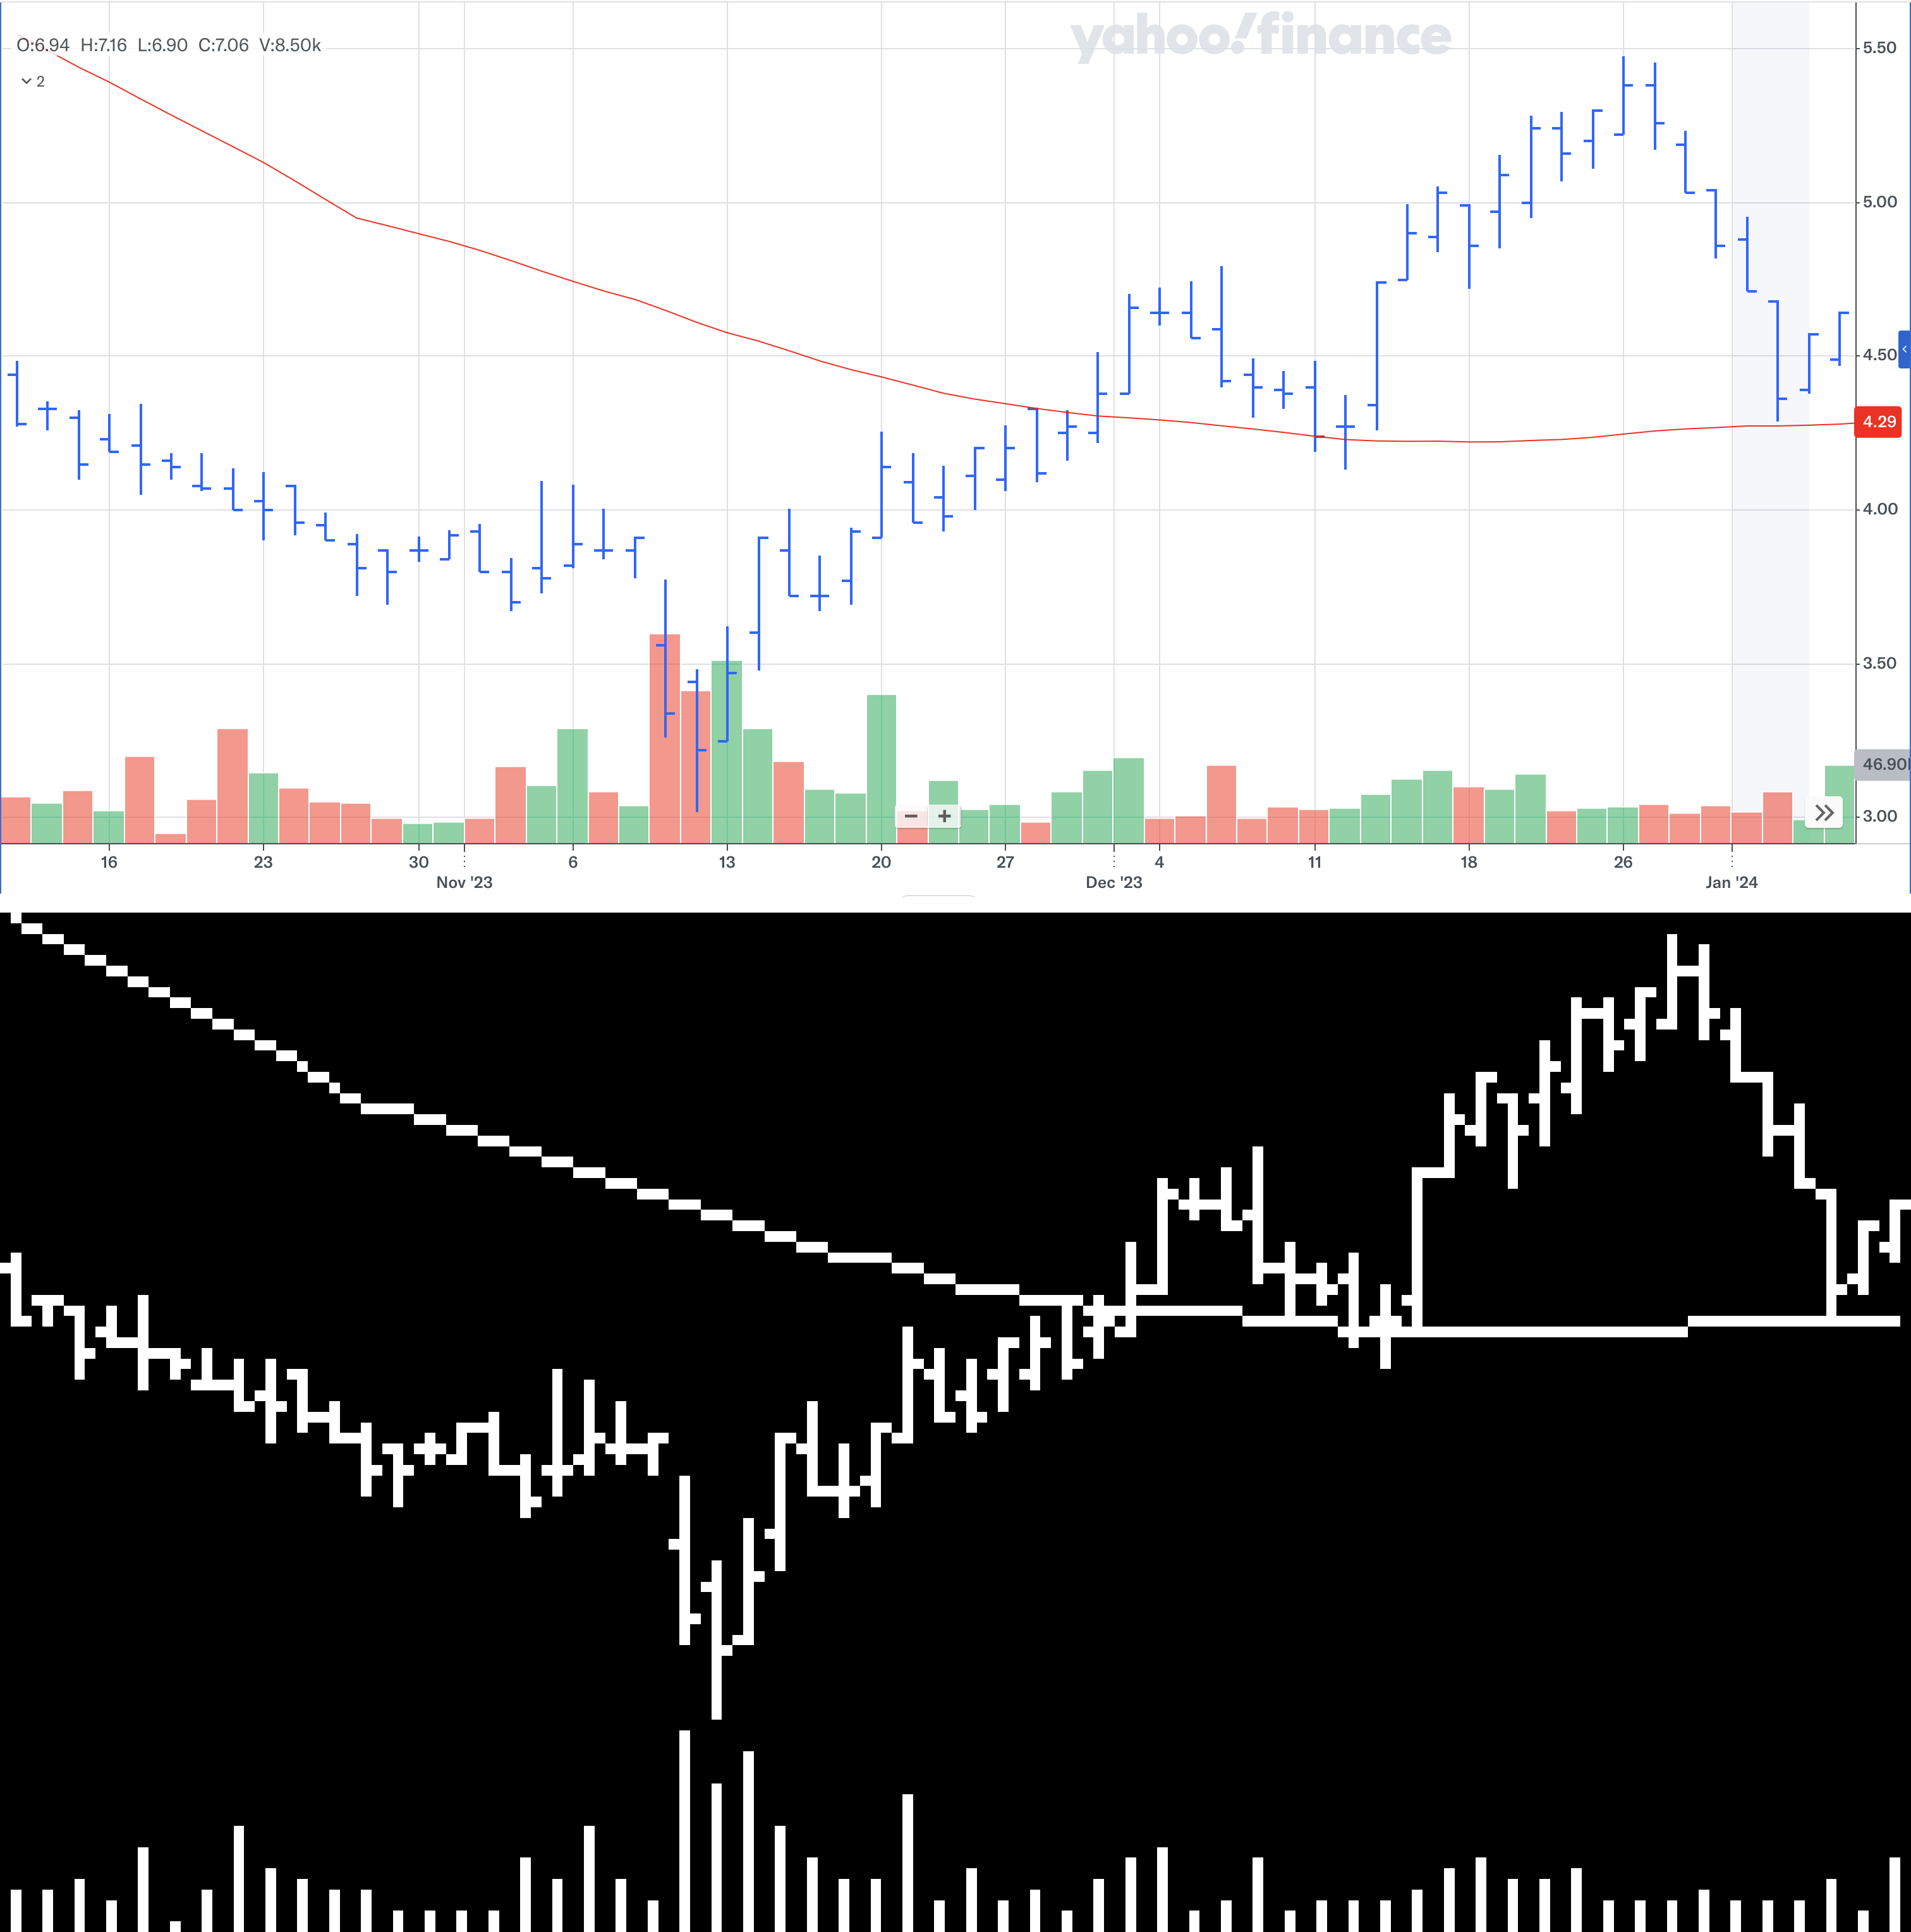
\includegraphics[width=0.82\textwidth]{chart_input_example.png}
\caption{Example of chart construction and model input. The upper panel shows a conventional OHLC-style chart, and the lower panel shows the corresponding binary grayscale input used by the chart CNN.}
\label{fig:chart_input}
\end{figure}

The sequence input uses the same market-history variables as ordered numerical channels. The six channels are open, high, low, close, moving average, and volume. The main CNN1D specification uses image-style scaling, where OHLC and moving-average values are jointly min-max scaled within the lookback window and volume is min-max scaled separately. We also evaluate cumulative-return scaling and devolatized-return scaling to isolate the role of normalization.

The chart CNN applies two-dimensional convolution to the image input. The CNN1D applies one-dimensional convolution along the time dimension of the sequence input. Both families use batch normalization, Leaky ReLU activations, pooling, dropout, cross-entropy loss, and the Adam optimizer. Architecture depth increases with input length. The multimodal model pairs chart and sequence inputs for the same stock-date observation and combines branch features before classification. We evaluate feature concatenation, a small MLP fusion head, and late fusion.

\subsection{Portfolio evaluation}

Each model or benchmark produces a stock-level score at formation date $t$. Stocks are sorted into deciles within each date. The high-minus-low portfolio buys the highest-score decile and shorts the lowest-score decile. We report equal-weighted and value-weighted portfolios. Weekly, monthly, and quarterly portfolios correspond to $R5$, $R20$, and $R60$ and use non-overlapping returns at the relevant frequency.

Gross returns are converted to net returns using a size-dependent one-way transaction-cost schedule. The cost is 10 basis points for stocks above the NYSE 80th-percentile market-capitalization breakpoint at the rebalancing date and 20 basis points otherwise. Costs are applied to traded notional in both legs. This adjustment captures turnover costs in a common way across learned models and benchmarks, while leaving market impact, borrowing costs, and capacity outside the direct trading model.

The benchmark set contains four price-based rules. Momentum uses the cumulative return from trading days $t-273$ through $t-22$. STR is the negative 21-day return. WSTR is the negative 5-day return. TREND combines normalized moving-average ratios over 3, 5, 10, 20, 50, 100, 200, 400, 600, 800, and 1000 trading days using rolling cross-sectional forecasting coefficients. These benchmarks span medium-horizon continuation, short-horizon reversal, and multi-horizon trend.

\section{Representation Results}

\subsection{Scaling}

Table~\ref{tab:scaling} compares chart CNN, logistic classifiers, and CNN1D under different sequence scaling schemes. The table reports annualized gross Sharpe ratios for high-minus-low decile portfolios over 2001--2024.

\begin{table}[htbp]
\centering
\scriptsize
\setlength{\tabcolsep}{4pt}
\renewcommand{\arraystretch}{0.96}
\caption{Portfolio performance across representation and scaling schemes}
\label{tab:scaling}
\begin{tabular*}{\textwidth}{@{\extracolsep{\fill}}lrrrrrr@{}}
\toprule
& \multicolumn{2}{c}{5-day inputs} & \multicolumn{2}{c}{20-day inputs} & \multicolumn{2}{c}{60-day inputs} \\
\cmidrule(lr){2-3}\cmidrule(lr){4-5}\cmidrule(l){6-7}
Model & EW & VW & EW & VW & EW & VW \\
\midrule
\multicolumn{7}{@{}c}{\textit{Five-day return horizon}} \\
\midrule
Chart CNN & 5.88 & 1.39 & 6.52 & 1.44 & 3.72 & 1.18 \\
Logistic, image scale & 4.88 & 1.25 & 5.22 & 1.09 & 5.44 & 1.12 \\
Logistic, cum. return scale & 0.18 & -0.04 & -0.41 & -0.51 & -0.26 & -0.53 \\
Logistic, devol. return scale & 2.80 & 0.79 & 2.73 & 0.48 & 2.70 & 0.66 \\
CNN1D, image scale & 6.24 & 1.16 & 6.55 & 1.12 & 5.89 & 2.06 \\
CNN1D, cum. return scale & 4.88 & 1.47 & 5.12 & 1.41 & 4.66 & 1.15 \\
CNN1D, devol. return scale & 4.39 & 0.73 & 5.26 & 1.04 & 4.82 & 1.28 \\
\addlinespace[3pt]
\midrule
\multicolumn{7}{@{}c}{\textit{20-day return horizon}} \\
\midrule
Chart CNN & 1.35 & 0.10 & 2.26 & 0.49 & 0.57 & -0.29 \\
Logistic, image scale & 2.03 & 0.56 & 2.37 & 0.41 & 1.59 & 0.60 \\
Logistic, cum. return scale & 0.02 & 0.37 & -0.29 & -0.08 & -0.30 & -0.64 \\
Logistic, devol. return scale & 1.27 & 0.59 & 1.02 & 0.28 & 0.98 & 0.12 \\
CNN1D, image scale & 2.18 & 0.41 & 2.15 & 0.41 & 1.74 & 0.51 \\
CNN1D, cum. return scale & 0.94 & 0.92 & 0.97 & 0.56 & 1.45 & 0.63 \\
CNN1D, devol. return scale & 1.17 & 0.16 & 1.73 & 0.53 & 1.22 & 0.30 \\
\addlinespace[3pt]
\midrule
\multicolumn{7}{@{}c}{\textit{60-day return horizon}} \\
\midrule
Chart CNN & 0.23 & -0.18 & 0.34 & 0.21 & 0.55 & 0.45 \\
Logistic, image scale & 0.97 & 0.04 & 0.94 & 0.21 & 0.55 & 0.21 \\
Logistic, cum. return scale & 0.37 & 0.11 & -0.02 & -0.06 & -0.30 & -0.54 \\
Logistic, devol. return scale & 0.66 & 0.08 & 0.61 & 0.37 & 0.40 & 0.17 \\
CNN1D, image scale & 0.99 & 0.28 & 0.46 & 0.15 & 0.46 & 0.25 \\
CNN1D, cum. return scale & 0.26 & 0.33 & 0.13 & 0.16 & 0.34 & 0.21 \\
CNN1D, devol. return scale & 0.83 & 0.13 & 0.65 & 0.34 & 0.45 & 0.21 \\
\bottomrule
\end{tabular*}
\caption*{\footnotesize The table reports annualized gross Sharpe ratios of high-minus-low decile spread portfolios over 2001--2024. EW and VW denote equal-weighted and value-weighted portfolios.}
\end{table}

The scaling choice is economically large. At the weekly horizon, image-scaled CNN1D reaches equal-weighted gross Sharpe ratios of 6.24, 6.55, and 5.89 across the three input windows, compared with 5.88, 6.52, and 3.72 for the chart CNN. The image-scaled logistic model also performs well relative to logistic classifiers based on cumulative-return and devolatized-return scaling. Local high-low normalization therefore carries substantial predictive content before nonlinear temporal learning is added.

CNN1D narrows differences across scaling schemes because flexible temporal learning extracts information from several encodings. The strongest comparison remains the image-scaled sequence, which removes the pixel layout while preserving the chart normalization. This sequence model recovers much of the chart-CNN edge.

\subsection{Fusion and overlap}

Figure~\ref{fig:fusion} compares multimodal fusion designs in the two strongest weekly settings. Feature concatenation, an MLP fusion head, and late fusion all perform well, but the relative ordering is unstable across samples and weighting schemes.

\begin{figure}[htbp]
\centering
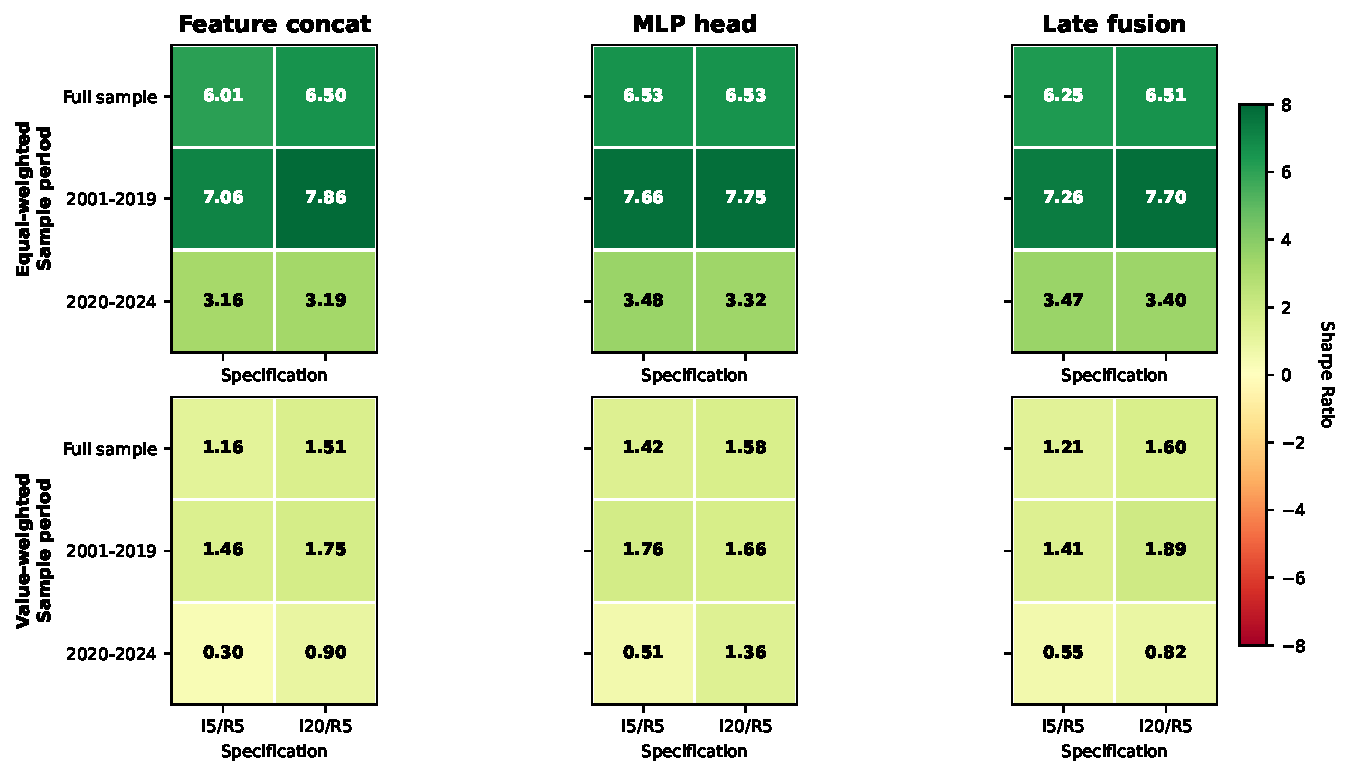
\includegraphics[width=\textwidth]{fusion_heatmap.pdf}
\caption{Gross Sharpe ratios for multimodal fusion designs in the strongest weekly specifications. The panels compare feature concatenation, an MLP fusion head, and late fusion across equal-weighted and value-weighted portfolios in the full sample, baseline sample, and extension sample.}
\label{fig:fusion}
\end{figure}

The fusion evidence supports a simple interpretation. Multimodal models are strong in the same regions where the single-branch models are strong. They do not create a stable new source of performance. This pattern is consistent with substantial overlap between the information extracted by chart and sequence branches.

Figure~\ref{fig:corr} reports date-level Spearman rank correlations between learned-model scores. The weekly cases have the highest overlap. In $I5/R5$ and $I20/R5$, chart CNN and CNN1D correlations are 0.73 and 0.67, and CNN1D and multimodal correlations are 0.84 and 0.80. The correlations are high enough to explain similar portfolio profiles, while remaining far from identical rankings.

\begin{figure}[htbp]
\centering
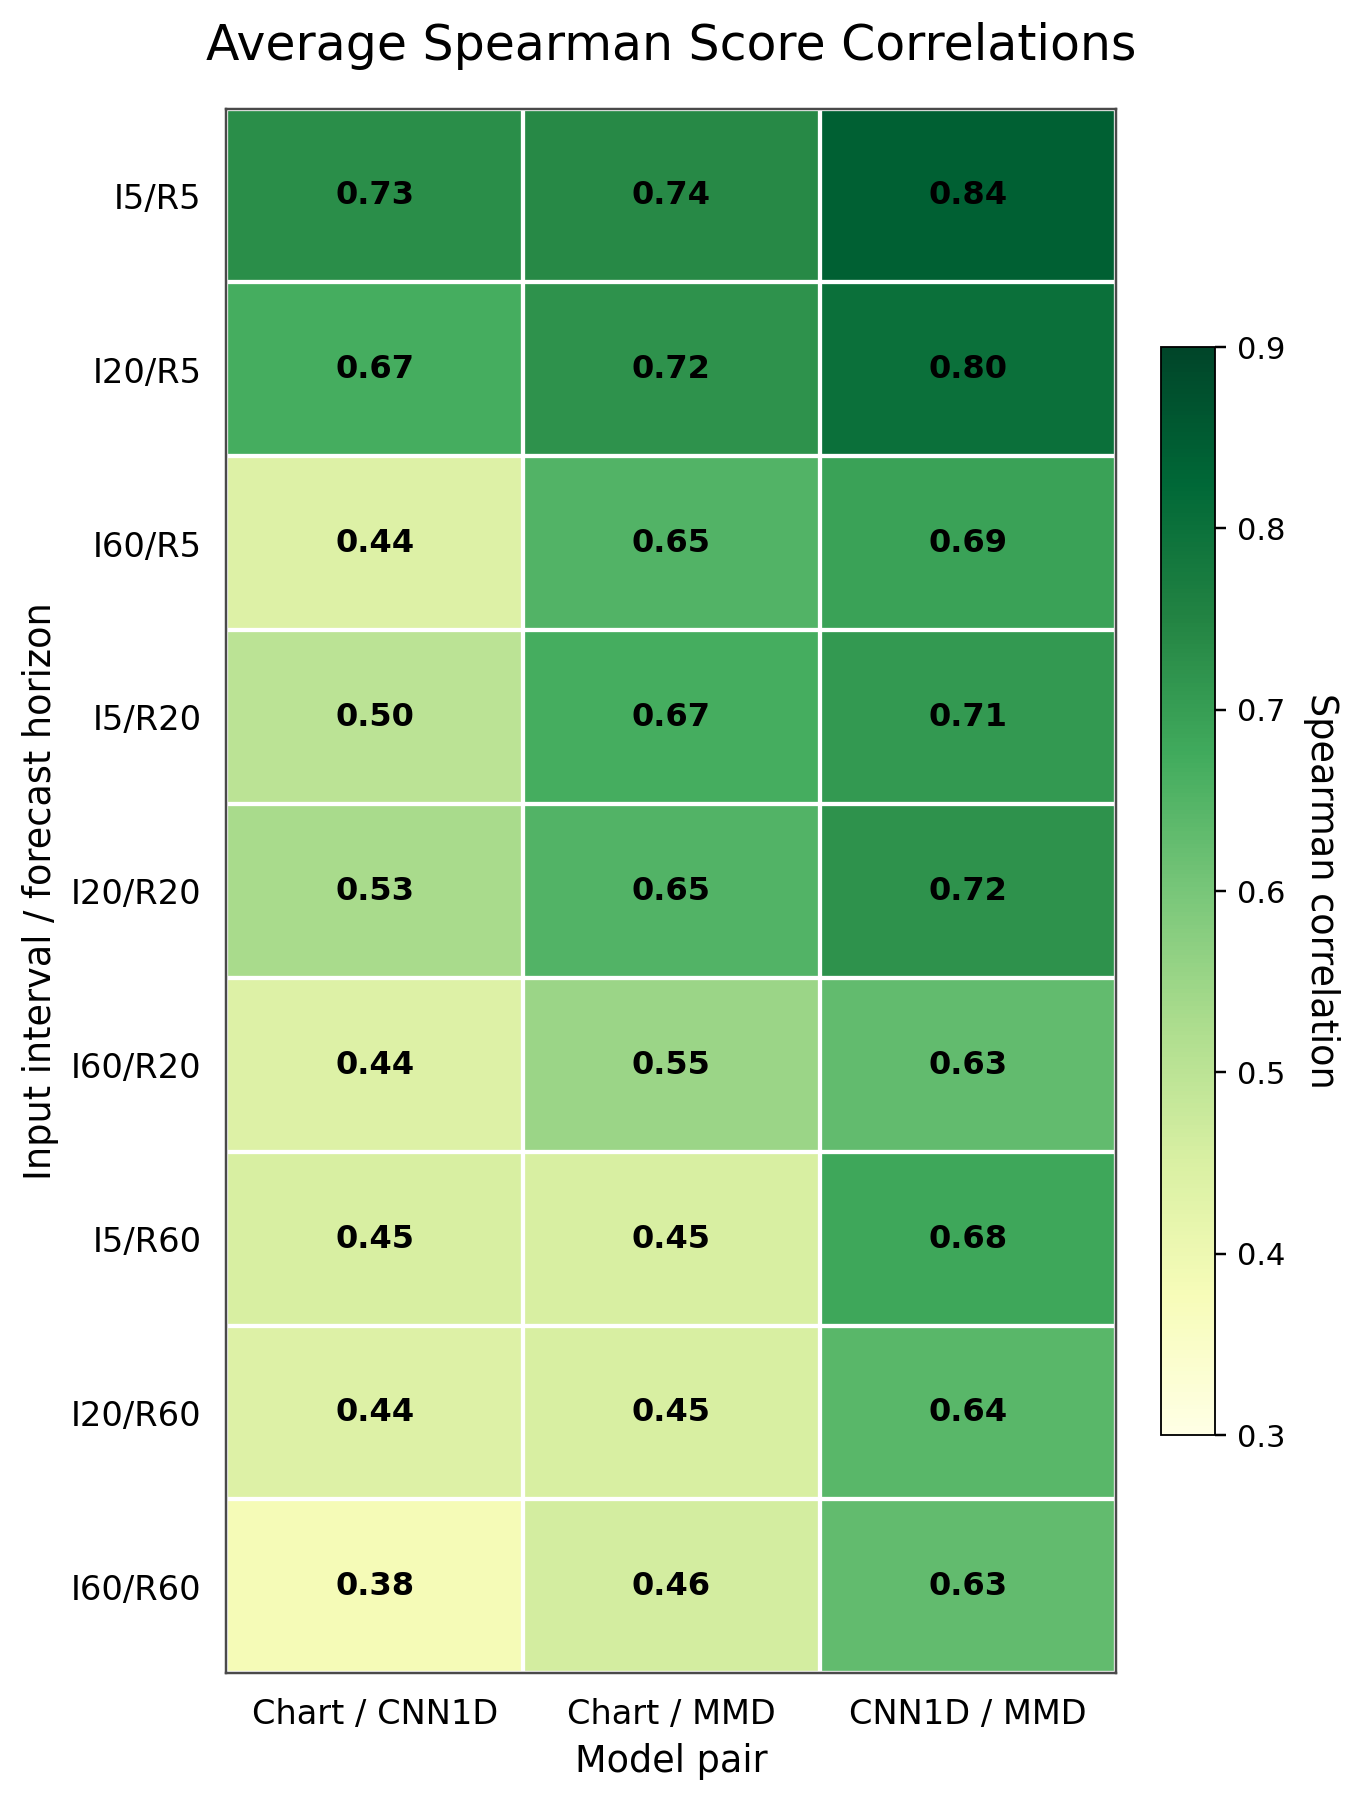
\includegraphics[width=0.78\textwidth]{score_correlation_heatmaps.png}
\caption{Average rank correlations between learned-model scores, 2001--2024. Each cell reports the average date-level Spearman correlation between pairs of learned-model scores on the common stock-date panel.}
\label{fig:corr}
\end{figure}

Table~\ref{tab:encompassing} adds conditional evidence. We regress future returns jointly on chart CNN, CNN1D, and multimodal scores using Fama--MacBeth cross-sectional regressions. CNN1D remains positive and significant throughout the grid. The chart CNN contributes in the strongest weekly and central monthly cases, while the multimodal score is less consistent once the two branches are included.

\begin{table}[htbp]
\centering
\scriptsize
\setlength{\tabcolsep}{6pt}
\caption{Encompassing regressions and incremental explanatory power}
\label{tab:encompassing}
\begin{tabular*}{\textwidth}{@{\extracolsep{\fill}}lrrrrrrr@{}}
\toprule
& \multicolumn{4}{c}{Joint regression $t$-statistics} & \multicolumn{3}{c}{Incremental $R^2$} \\
\cmidrule(lr){2-5}\cmidrule(l){6-8}
Spec. & Chart CNN & CNN1D & Multimodal & Avg. $R^2$ & Add 1D & Add 2D & Add MM \\
\midrule
$I5/R5$ & \(6.95^{***}\) & \(12.56^{***}\) & \(8.39^{***}\) & 0.70 & 0.13 & 0.15 & 0.05 \\
$I20/R5$ & \(9.51^{***}\) & \(11.80^{***}\) & \(11.91^{***}\) & 0.80 & 0.22 & 0.12 & 0.08 \\
$I60/R5$ & -1.12 & \(18.19^{***}\) & \(9.95^{***}\) & 0.95 & 0.44 & 0.11 & 0.13 \\
$I5/R20$ & -0.26 & \(4.39^{***}\) & -0.73 & 0.52 & 0.15 & 0.07 & 0.19 \\
$I20/R20$ & \(3.93^{***}\) & \(5.76^{***}\) & \(3.36^{***}\) & 0.65 & 0.27 & 0.09 & 0.10 \\
$I60/R20$ & -0.85 & \(4.66^{***}\) & 0.28 & 1.06 & 0.79 & 0.09 & 0.11 \\
$I5/R60$ & -0.74 & \(2.16^{**}\) & \(2.56^{**}\) & 0.50 & 0.22 & 0.20 & 0.05 \\
$I20/R60$ & -0.50 & \(2.83^{***}\) & 1.37 & 0.75 & 0.28 & 0.15 & 0.09 \\
$I60/R60$ & -0.46 & \(3.97^{***}\) & 0.71 & 1.13 & 0.45 & 0.20 & 0.11 \\
\bottomrule
\end{tabular*}
\caption*{\footnotesize The first three columns report Fama--MacBeth $t$-statistics from joint regressions with all three learned scores. Stars denote two-sided significance: $^{*}p<0.10$, $^{**}p<0.05$, and $^{***}p<0.01$. Avg. $R^2$ is expressed in percent. Incremental $R^2$ entries are percentage-point increases from adding the named score. Add MM adds the multimodal score after both single-branch scores.}
\end{table}

The regression evidence reconciles the representation results. The portfolios look similar because the models recover a common broad short-horizon ranking signal. The representations remain distinct enough that CNN1D contributes stable incremental content and the chart CNN contributes in selected short-horizon cases. The multimodal model mainly recombines information already present in the two branches.

\section{Economic Performance and Implementation}

\subsection{Benchmarks and costs}

Before costs, learned models outperform price-based benchmarks most clearly in equal-weighted weekly portfolios. In the full 2001--2024 sample, the $I20/R5$ chart CNN, CNN1D, and multimodal models have gross Sharpe ratios of 6.52, 6.55, and 6.48. WSTR and TREND are meaningful weekly benchmarks, with gross Sharpe ratios of 2.86 and 2.49, while MOM is weak in this comparison. The advantage narrows at monthly and quarterly horizons and under value-weighting.

Figure~\ref{fig:netheat} shows net Sharpe ratios after transaction costs over the learned-model grid. Net performance is concentrated in the equal-weighted weekly region. CNN1D and the multimodal model are especially strong at longer input windows, while value-weighted net results are much smaller.

\begin{figure}[htbp]
\centering
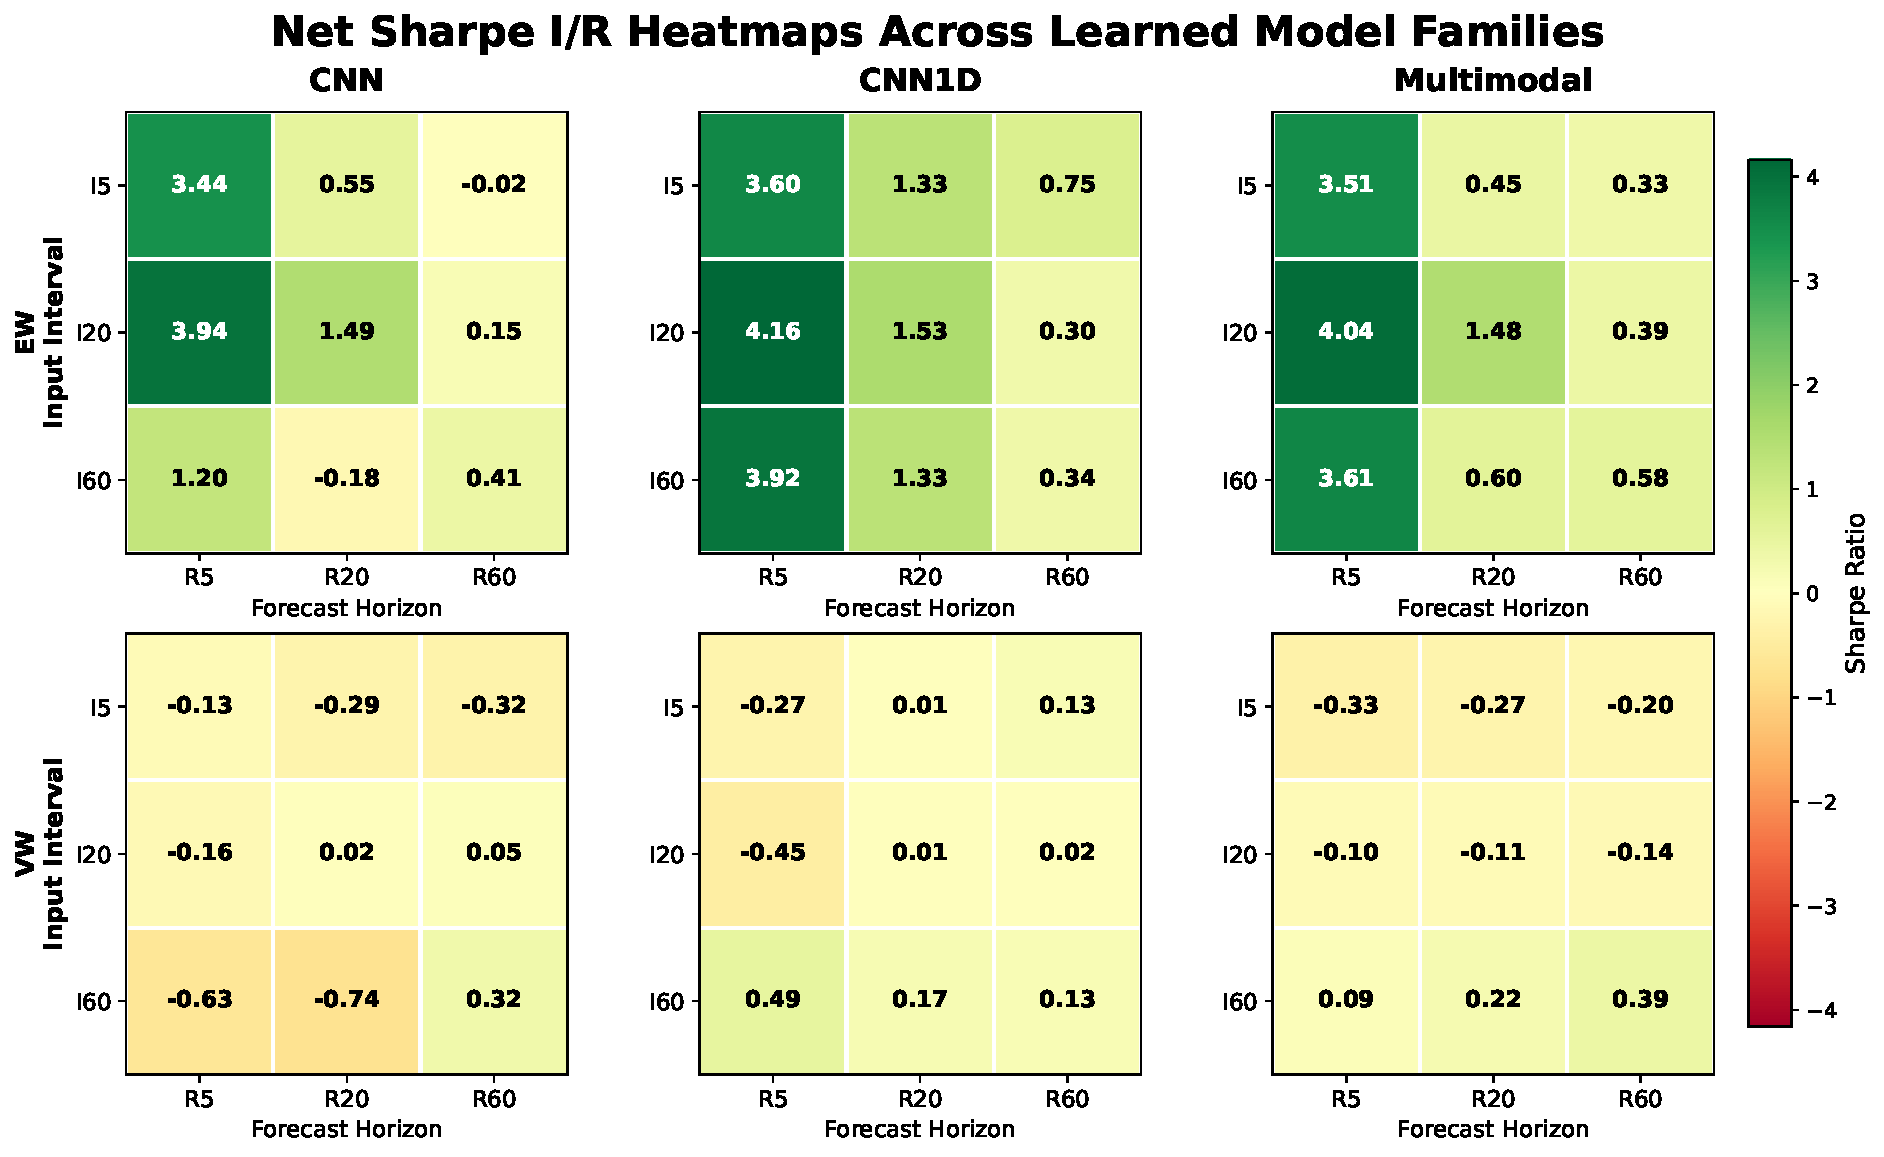
\includegraphics[width=\textwidth]{fullsample_net_sr_heatmaps.pdf}
\caption{Full-sample net Sharpe-ratio heatmaps over the $I/R$ grid for the three learned model families. The panels report 2001--2024 net Sharpe ratios after transaction costs, separated by portfolio weighting scheme.}
\label{fig:netheat}
\end{figure}

Figure~\ref{fig:cumnet} plots cumulative volatility-adjusted net log returns for the representative $I20/R5$ weekly comparison. Transaction costs reduce the level of all active strategies, but the learned models remain clearly above the benchmark strategies in the full equal-weighted universe.

\begin{figure}[htbp]
\centering
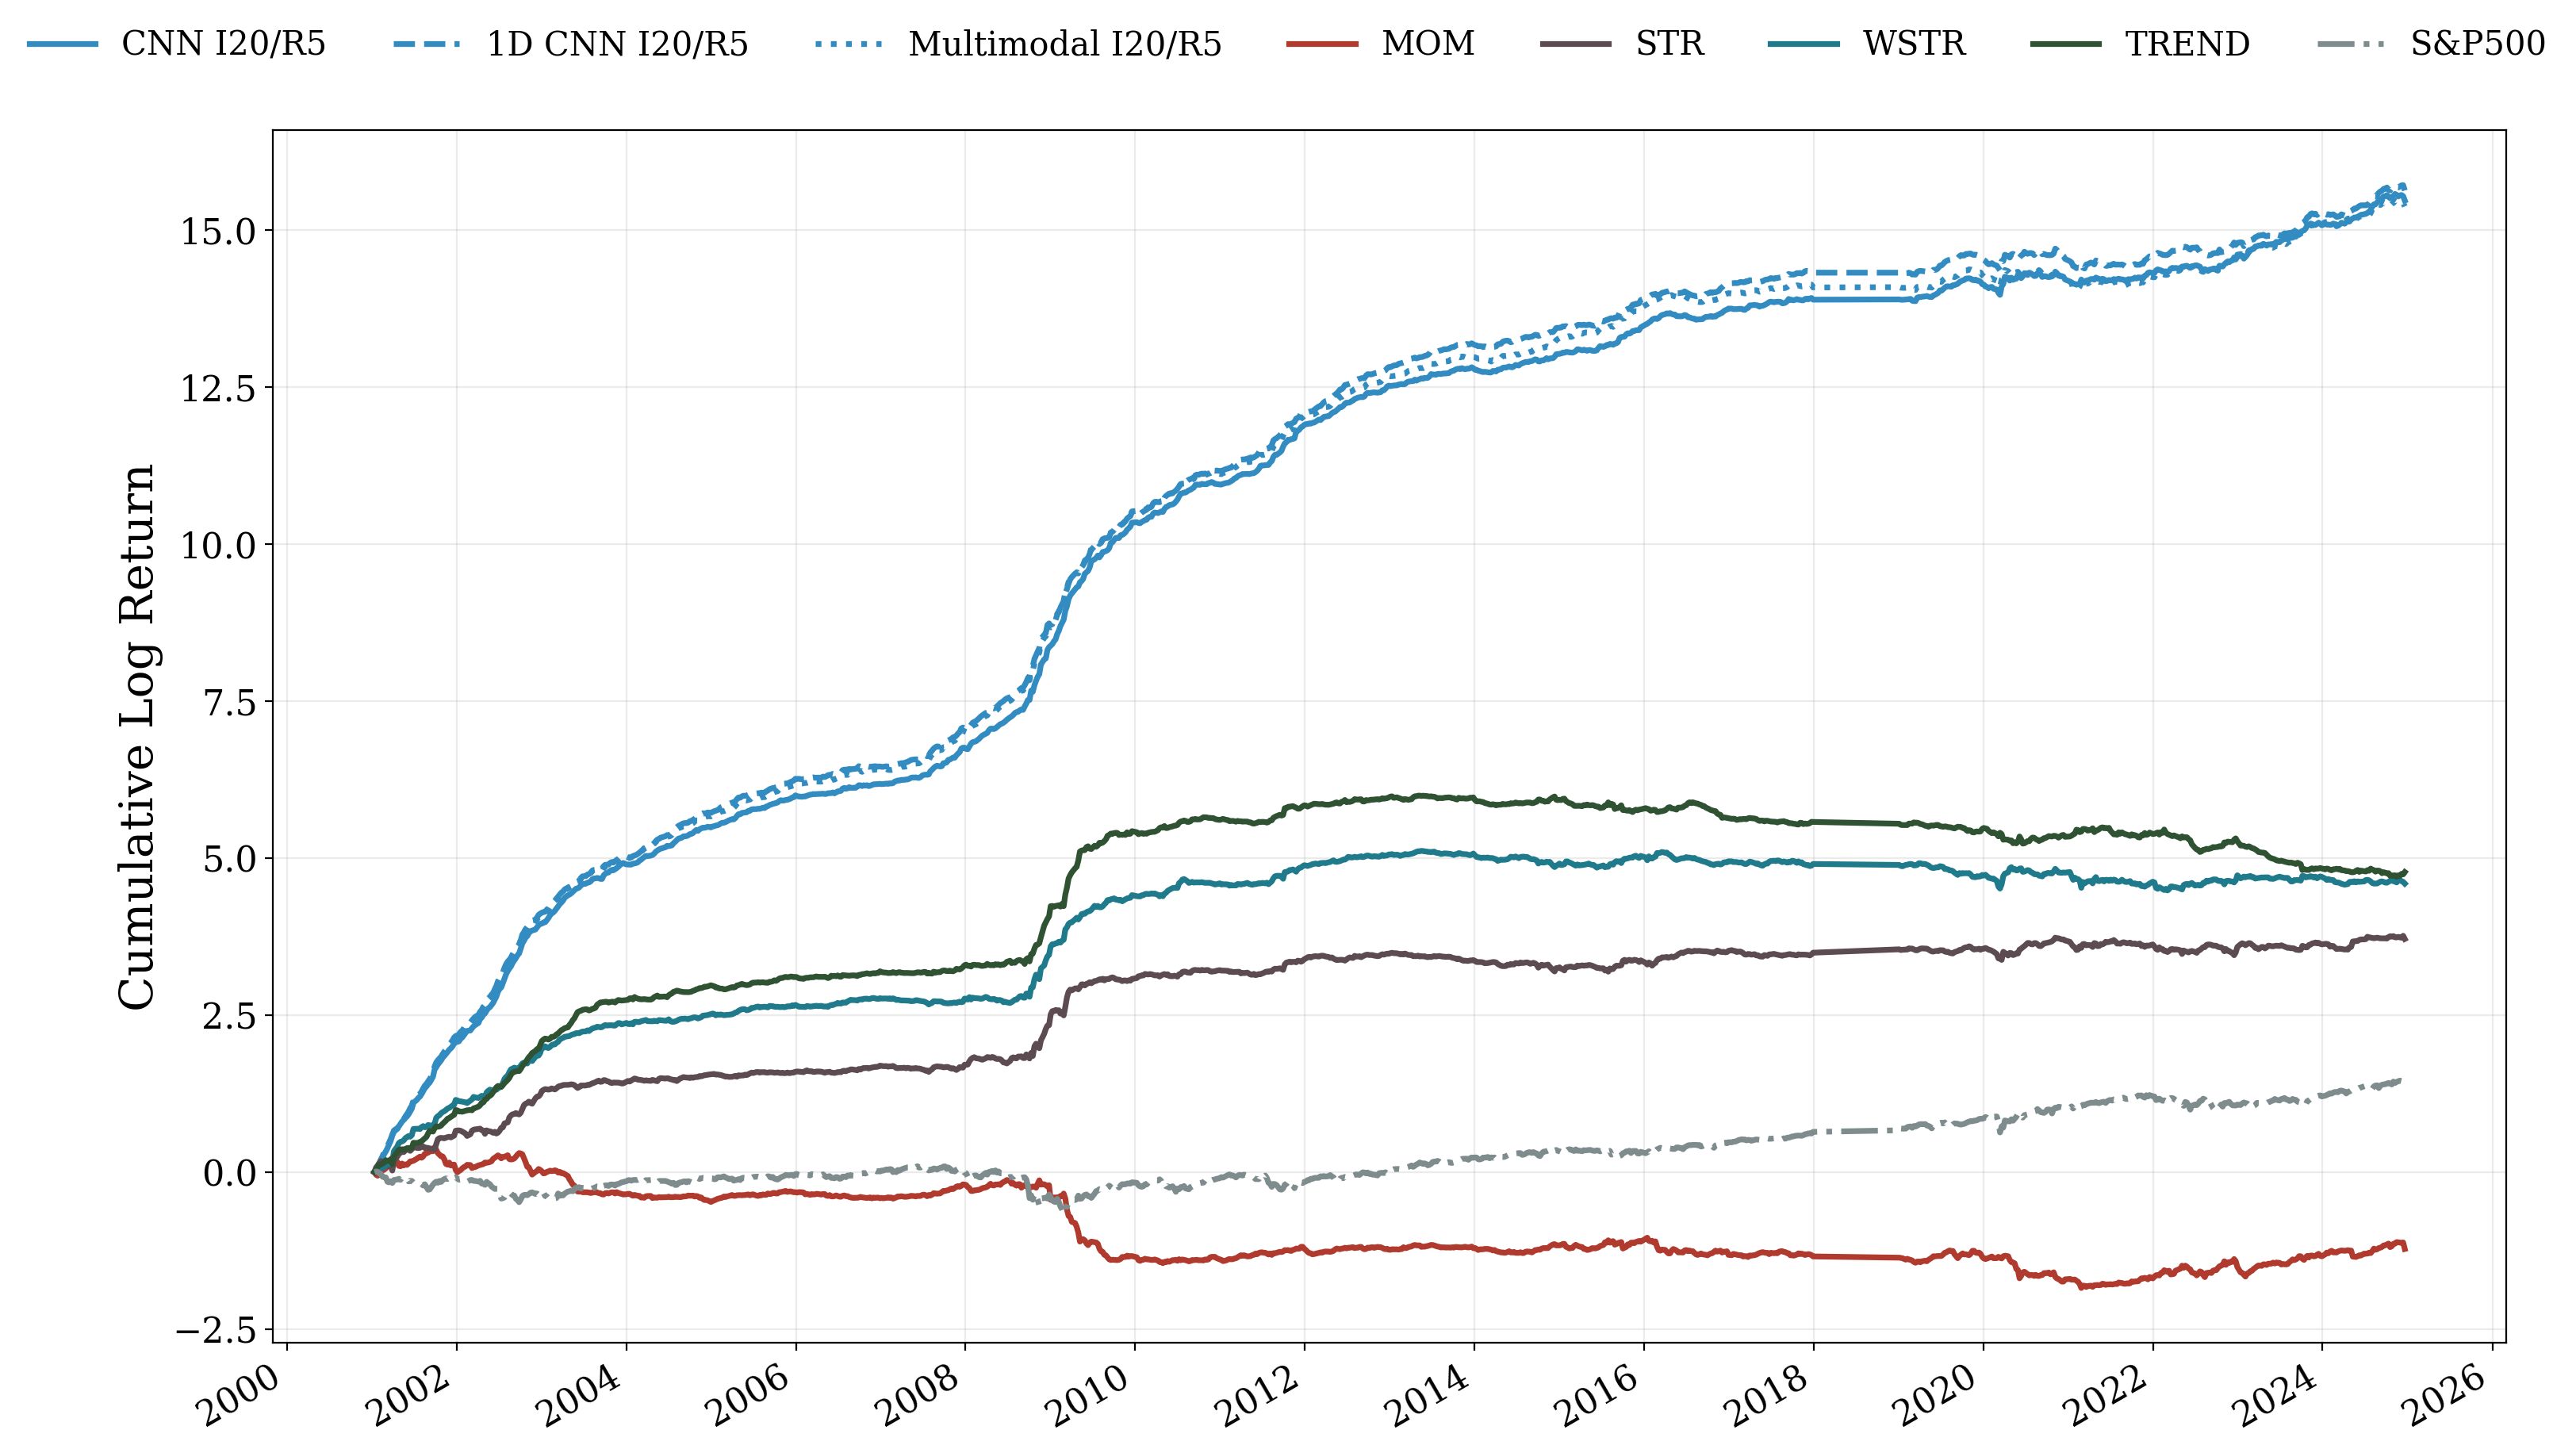
\includegraphics[width=\textwidth]{fullsample_cumulative_net.png}
\caption{Cumulative volatility-adjusted net log returns for the $I20/R5$ learned models, benchmark strategies, and the S\&P 500, 2001--2024.}
\label{fig:cumnet}
\end{figure}

\subsection{Tradability and factor adjustment}

Table~\ref{tab:tradability} examines the representative weekly $I20/R5$ portfolios under stricter tradability filters and Carhart factor adjustment. The full-universe portfolios retain large annualized net alphas. The same portfolios become negative under dollar-volume, no-microcap, and combined filters.

\begin{table}[htbp]
\centering
\scriptsize
\setlength{\tabcolsep}{3pt}
\renewcommand{\arraystretch}{0.88}
\caption{Representative weekly tradability and factor diagnostics}
\label{tab:tradability}
\begin{tabular*}{\textwidth}{@{\extracolsep{\fill}}llrrrrrr@{}}
\toprule
Model & Filter & Net Ret. & Net SR & Carhart $\alpha$ & $t(\alpha)$ & Names & Turn. \\
\midrule
\multicolumn{8}{@{}l}{\textit{Panel A: Chart CNN}} \\
 & Full & 51.3\% & 3.94 & 49.3\% & 11.81 & 420 & 6.65 \\
 & Price & 10.1\% & 1.08 & 8.1\% & 3.67 & 321 & 6.66 \\
 & DV \$1m & -10.0\% & -0.85 & -11.0\% & -3.87 & 241 & 7.01 \\
 & DV \$5m & -19.5\% & -1.57 & -20.6\% & -7.27 & 164 & 7.07 \\
 & No microcaps & -17.0\% & -1.60 & -18.1\% & -7.38 & 193 & 6.89 \\
 & Combined & -22.9\% & -2.10 & -24.0\% & -10.21 & 149 & 7.02 \\
\addlinespace[1pt]
\multicolumn{8}{@{}l}{\textit{Panel B: CNN1D}} \\
 & Full & 56.5\% & 4.16 & 55.2\% & 12.56 & 419 & 6.46 \\
 & Price & 13.7\% & 1.48 & 12.4\% & 5.46 & 319 & 6.50 \\
 & DV \$1m & -5.7\% & -0.46 & -6.2\% & -2.21 & 240 & 6.68 \\
 & DV \$5m & -15.0\% & -1.17 & -15.7\% & -5.61 & 164 & 6.75 \\
 & No microcaps & -14.8\% & -1.37 & -15.6\% & -6.34 & 192 & 6.57 \\
 & Combined & -19.0\% & -1.68 & -19.8\% & -8.11 & 149 & 6.69 \\
\addlinespace[1pt]
\multicolumn{8}{@{}l}{\textit{Panel C: Multimodal}} \\
 & Full & 54.5\% & 4.04 & 53.2\% & 12.10 & 419 & 6.56 \\
 & Price & 13.5\% & 1.52 & 12.4\% & 5.46 & 319 & 6.63 \\
 & DV \$1m & -5.2\% & -0.42 & -5.5\% & -1.91 & 240 & 6.83 \\
 & DV \$5m & -14.1\% & -1.11 & -14.7\% & -5.12 & 164 & 6.92 \\
 & No microcaps & -14.0\% & -1.33 & -14.6\% & -5.85 & 192 & 6.75 \\
 & Combined & -19.3\% & -1.76 & -19.9\% & -8.32 & 149 & 6.87 \\
\bottomrule
\end{tabular*}
\caption*{\footnotesize Net Ret. denotes annualized net return, Carhart $\alpha$ is annualized, Names is the average number of stocks per side, and Turn. denotes monthly-equivalent average turnover. Price requires a price of at least \$5. DV filters require dollar volume of at least \$1 million or \$5 million. No microcaps excludes stocks below the NYSE 20th percentile market-cap breakpoint. Combined applies the no-microcap, price, and DV \$5m filters jointly.}
\end{table}

The table separates factor exposure from tradability. Standard market, size, value, and momentum factors do not explain the full-universe weekly net returns. The liquidity and size screens remove most of the economic performance. Predictability is therefore broader than factor exposure, while implementable value is concentrated in the broad equal-weighted universe and depends heavily on less liquid stocks.

\section{Sample Stability}

The 2020--2024 extension period is a direct stress test for learned return prediction from recent market histories. Figure~\ref{fig:extnet} plots cumulative volatility-adjusted net log returns for the representative weekly portfolios during this period. The learned models remain positive in this specification, but the paths are less smooth and the scale is much smaller than in the full sample.

\begin{figure}[htbp]
\centering
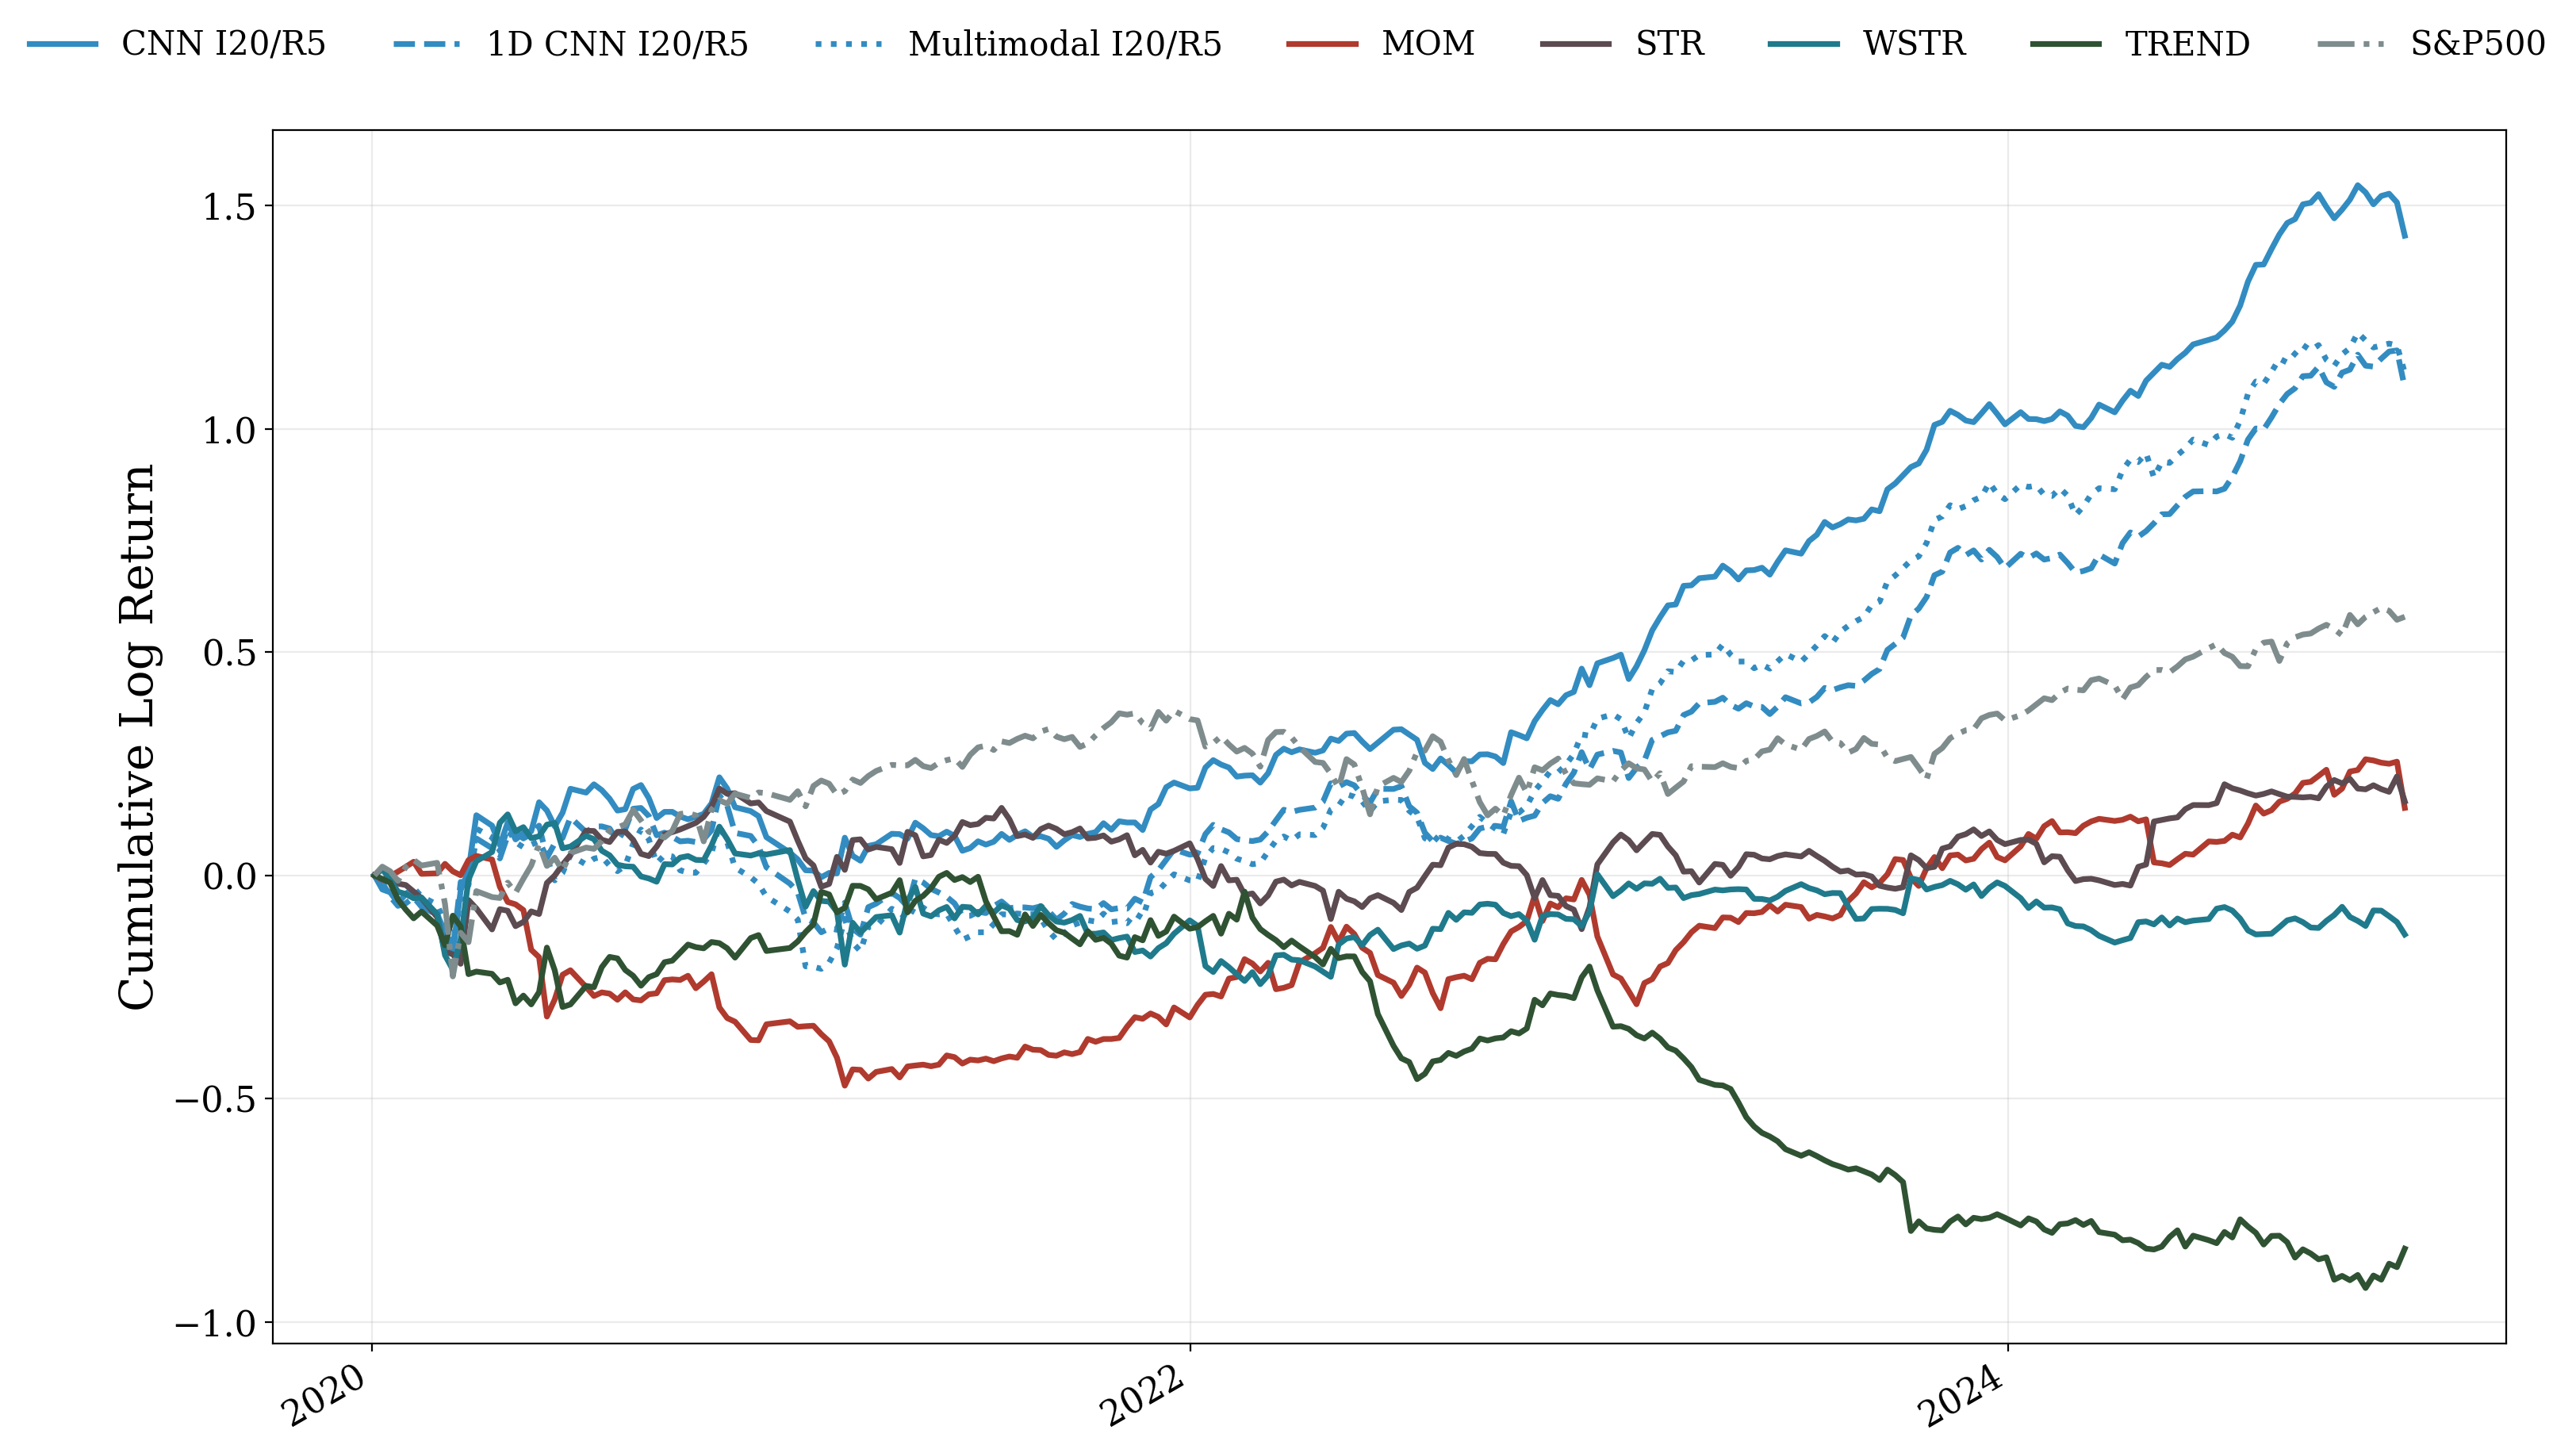
\includegraphics[width=\textwidth]{extension_cumulative_net.png}
\caption{Extension-period cumulative volatility-adjusted net log returns, 2020--2024. The figure reports cumulative net performance for learned models, benchmark strategies, and the S\&P 500 under the same portfolio construction and transaction cost assumptions as in the full-sample analysis.}
\label{fig:extnet}
\end{figure}

Table~\ref{tab:best} summarizes the best equal-weighted learned specification and the best benchmark by period and horizon. The baseline rows show a large learned-model advantage, especially at the weekly horizon. The extension rows show weaker but still positive learned-model performance, with smaller margins over the best benchmarks.

\begin{table}[htbp]
\centering
\scriptsize
\setlength{\tabcolsep}{3pt}
\renewcommand{\arraystretch}{0.98}
\caption{Best equal-weighted learned model and benchmark by period and horizon}
\label{tab:best}
\resizebox{\textwidth}{!}{%
\begin{tabular}{@{}lllrrrlrrr@{}}
\toprule
 & & \multicolumn{4}{c}{Best learned model} & \multicolumn{4}{c}{Best benchmark} \\
\cmidrule(lr){3-6}\cmidrule(l){7-10}
Period & Horizon & Learned spec. & Net Ret. & Net SR & Turn. & Benchmark & Net Ret. & Net SR & Turn. \\
\midrule
2001--2019 & Weekly & CNN1D $I60/R5$ & 71.78\% & 5.58 & 5.98 & TREND & 38.27\% & 1.85 & 5.13 \\
2001--2019 & Monthly & CNN1D $I20/R20$ & 21.67\% & 1.92 & 1.73 & WSTR & 12.26\% & 0.87 & 1.67 \\
2001--2019 & Quarterly & CNN1D $I5/R60$ & 9.02\% & 0.83 & 0.59 & STR & 5.17\% & 0.22 & 0.55 \\
\addlinespace[2pt]
2020--2024 & Weekly & Chart CNN $I20/R5$ & 18.53\% & 1.35 & 6.65 & STR & 11.02\% & 0.44 & 3.27 \\
2020--2024 & Monthly & Chart CNN $I20/R20$ & 19.60\% & 1.30 & 1.75 & TREND & 5.52\% & 0.30 & 1.17 \\
2020--2024 & Quarterly & CNN1D $I5/R60$ & 6.49\% & 0.51 & 0.60 & TREND & 7.11\% & 0.43 & 0.42 \\
\bottomrule
\end{tabular}%
}
\caption*{\footnotesize The table selects the highest net Sharpe ratio within each period-horizon block from the equal-weighted learned-model and benchmark grids. Turn. denotes monthly-equivalent average turnover.}
\end{table}

Figure~\ref{fig:scatter} compares chart and sequence performance across the baseline and extension periods. The baseline panel shows the strongest chart CNN and CNN1D specifications in the same high-performance region. The extension panel has a much lower scale, and representation rankings change across cells. Multimodal gains over the better single branch are usually small.

\begin{figure}[htbp]
\centering
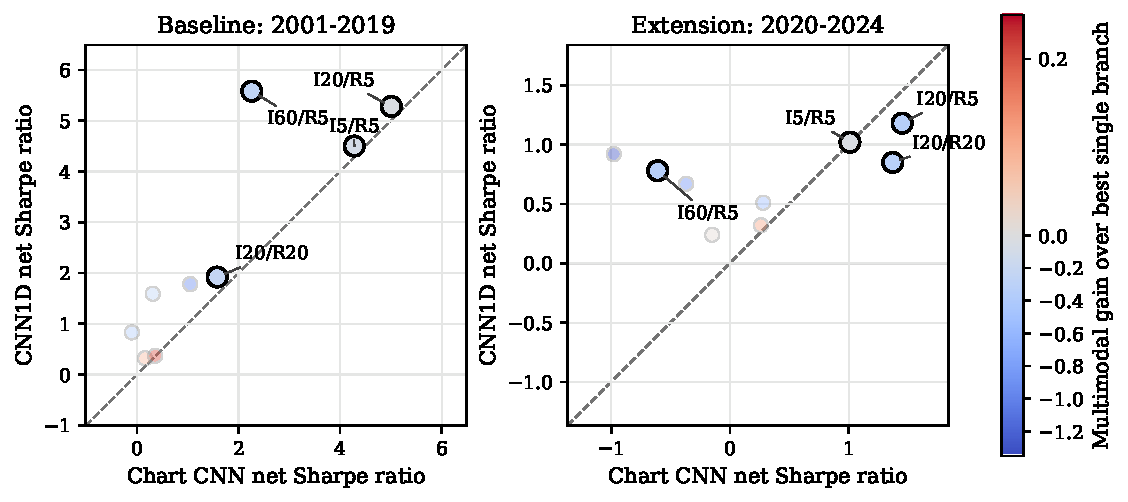
\includegraphics[width=\textwidth]{representation_scatter.pdf}
\caption{Equal-weighted net Sharpe ratios for chart and sequence representations across $I/R$ specifications. The horizontal axis reports chart CNN net Sharpe ratios, the vertical axis reports CNN1D net Sharpe ratios, and the color reports the multimodal net-Sharpe gain over the stronger single-branch model.}
\label{fig:scatter}
\end{figure}

The sample split changes the strength of the result without changing the interpretation. Chart and sequence inputs both recover short-horizon signals. CNN1D provides the most stable incremental content. Multimodal fusion remains competitive but rarely improves materially on the better branch. The extension period makes the economic value more conditional.

\section{Conclusion}

We study whether chart-based return prediction reflects visual information in the chart image or flexible learning from locally normalized recent market histories. The evidence points to local scaling plus temporal learning as the main channel behind much of the chart-CNN edge.

The chart CNN is an effective short-horizon predictor. A CNN1D trained on the same locally scaled market-history window recovers most of its performance and contributes the most consistent incremental content in regression diagnostics. Multimodal fusion performs strongly in the same regions, with limited gains over the best single branch. The learned models therefore share a broad short-horizon ranking signal, with representation-specific variation around that common component.

Benchmark comparisons give the signal its economic scale. Learned models outperform momentum, short-horizon reversal, and trend benchmarks most clearly in equal-weighted weekly portfolios. The edge narrows under transaction costs, value-weighting, stricter tradability screens, and newer data. Full-universe weekly returns retain large Carhart-adjusted alphas, but the performance turns negative under dollar-volume and no-microcap restrictions. The signal is real in the broad cross-section and much harder to interpret as scalable trading performance.

The main contribution is a controlled representation design. Holding the market-history window, horizon, ranking rule, portfolio construction, costs, and sample split fixed lets us ask what changes when the same recent price and volume path is represented as an image, a sequence, or a fused input. Under that design, chart images are one effective representation among several for a locally scaled market-history signal. The empirical value of the signal depends on costs, liquidity, weighting, and sample period.

\section*{Data Availability}

The empirical analysis uses CRSP daily equity data and Kenneth R. French factor data. CRSP data are available through institutional subscription. Code and derived non-proprietary artifacts can be organized for replication subject to data-license restrictions.

\section*{Declaration of Generative AI and AI-Assisted Technologies}

During manuscript preparation, the authors used OpenAI Codex to assist with drafting, editing, and LaTeX assembly. The authors reviewed and edited the content and take full responsibility for the manuscript.

\printbibliography

\end{document}
